\documentclass[11pt, twoside, pdftex]{article}

% This includes all the settings that we should use for the document
\newcommand{\PDFTitle}{Altera FPGA University Program Audio Core}
\newcommand{\commonPath}{../../Common}
\input{\commonPath/Docs/defaulttext.tex}
\input{\commonPath/Docs/preamble.tex}

\usepackage{placeins}

%%%%%%%%%%%%%%%%%%%%%%%%%
% Add title
\newcommand{\doctitle}{Audio core for \\ Altera\textsuperscript{\textregistered} DE-Series Boards}
\newcommand{\dochead}{Audio core for \\ Altera\textsuperscript{\textregistered} DE-Series Boards}
% Usually no need to change these two lines
\title{\fontfamily{phv}\selectfont{\doctitle} }
\chead{ \small{\textsc{\bfseries \dochead} } }
% Customizations
%%%%%%%%%%%%%%%%%%%%%%%%%
% Allows multiple figures per page

\renewcommand\floatpagefraction{.9}
\renewcommand\topfraction{.9}
\renewcommand\bottomfraction{.9}
\renewcommand\textfraction{.1}   
\setcounter{totalnumber}{50}
\setcounter{topnumber}{50}
\setcounter{bottomnumber}{50}
\raggedbottom
% Customizations
%%%%%%%%%%%%%%%%%%%%%%%%%

\begin{document}
\begin{table}
    \centering
    \begin{tabular}{p{5cm}p{4cm}}
        \hspace{-3.5cm}\includegraphics[width=0.4\textwidth]{\commonPath/Figures/altera.png}
        &
        \raisebox{1\height}{\parbox[h]{0.5\textwidth}{\Large\fontfamily{phv}\selectfont{\textsf{\doctitle}}}}
    \end{tabular}
    \label{tab:logo}
\end{table}
%\begin{table}
   % \centering
    %\begin{tabular}{p{5cm}p{4cm}}
    %    \hspace{-3.5cm}\includegraphics[width=0.4\textwidth]{\headerLogoFilePath{\UPTemplatePath/Figures}}
    %    &
    %    \raisebox{1\height}{\parbox[h]{0.4\textwidth}{\Large\fontfamily{phv}\selectfont{\textbf{\doctitle}}}}
    %\end{tabular}
    %\label{tab:logo}
%\end{table}

\colorbox[rgb]{0,0.384,0.816}{\parbox[h]{\textwidth}{\color{white}\textbf{\textit{\textBar}}}}

\thispagestyle{plain}

\section{Core Overview}
%    * Describe the function of the core, from a system-level perspective, at a very high level.
%    * Explain why this component exists. What type of problem was the core created to solve?
%    * List major features of the core.
%    * List approximate resource usage & performance for a basic configuration
%    (if appropriate). Note that if the size of the core differs wildly,
%    depending on the configuration, it's better to not set expectations one
%    way or the other. Or, state a range, and make it clear that "your mileage
%    will vary."
%    * Note significant differences from other similar cores (if applicable).
The Audio core interacts with the Audio CODEC (enCOder/DECoder) on
the Altera\textsuperscript{\textregistered} DE-series boards and provides an interface for audio input
and output.

\section{Functional Description}
%    *  This section describes the hardware structure of the core, and how it functions.
%    * Show a block diagram of the core. For cores that vary in shape depending
%    on parameters, you might have to show a typical or a maximal
%    configuration. List the input and output signals of the core.
%    * Describe each functional unit of the core hardware.
%    * If possible, include a high-level narrative of how the core operates in
%    a system. I.e., "Data comes from point A. The core processes it in
%    functional unit B. The core sends processed data out to point C." Each
%    functional unit of the core can contain some narrative about how it
%    behaves in a system.
The Audio core facilitates the transfer of audio data with the Audio CODEC chip
on the Altera DE-series boards. Data is transferred serially between the FPGA 
and the CODEC. However, data written/read to/from the Audio core is transfered 
in a parallel manner. The Audio core automatically serializes/deserializes the 
data. 

The Audio core contains four FIFOs to buffer the In and Out 
audio data, both having the right and left audio channels. Each FIFO can store 
up to 128 32-bit words. To guarantee that the left and right audio output 
channels are synchronized, data will not play until both channels are received. 
If only one channel is to be played, the other channel must have zeros written 
to it. 

The Audio core can be connected to a system using one of two different modes:
Memory-Mapped or Streaming. Figure~\hyperref[fig:blockdiagrammm]{1} shows a 
block diagram of the Audio core with a memory-mapped interface. This mode 
allows access to the core's FIFOs through memory-mapped registers. This is
suitable when connecting the core to a processor, such as the Nios\textsuperscript{\textregistered} II processor,
using the Platform Designer System Integration tool.
Figure~\hyperref[fig:blockdiagramst]{2} shows a block diagram of the Audio core 
with a streaming interface. This mode allows direct access to the core's FIFOs.
This is suitable when connecting to custom hardware using the Platform Designer System 
Integration tool or as a standalone component using the IP Catalog.

\begin{figure}[h]
    \begin{center}
        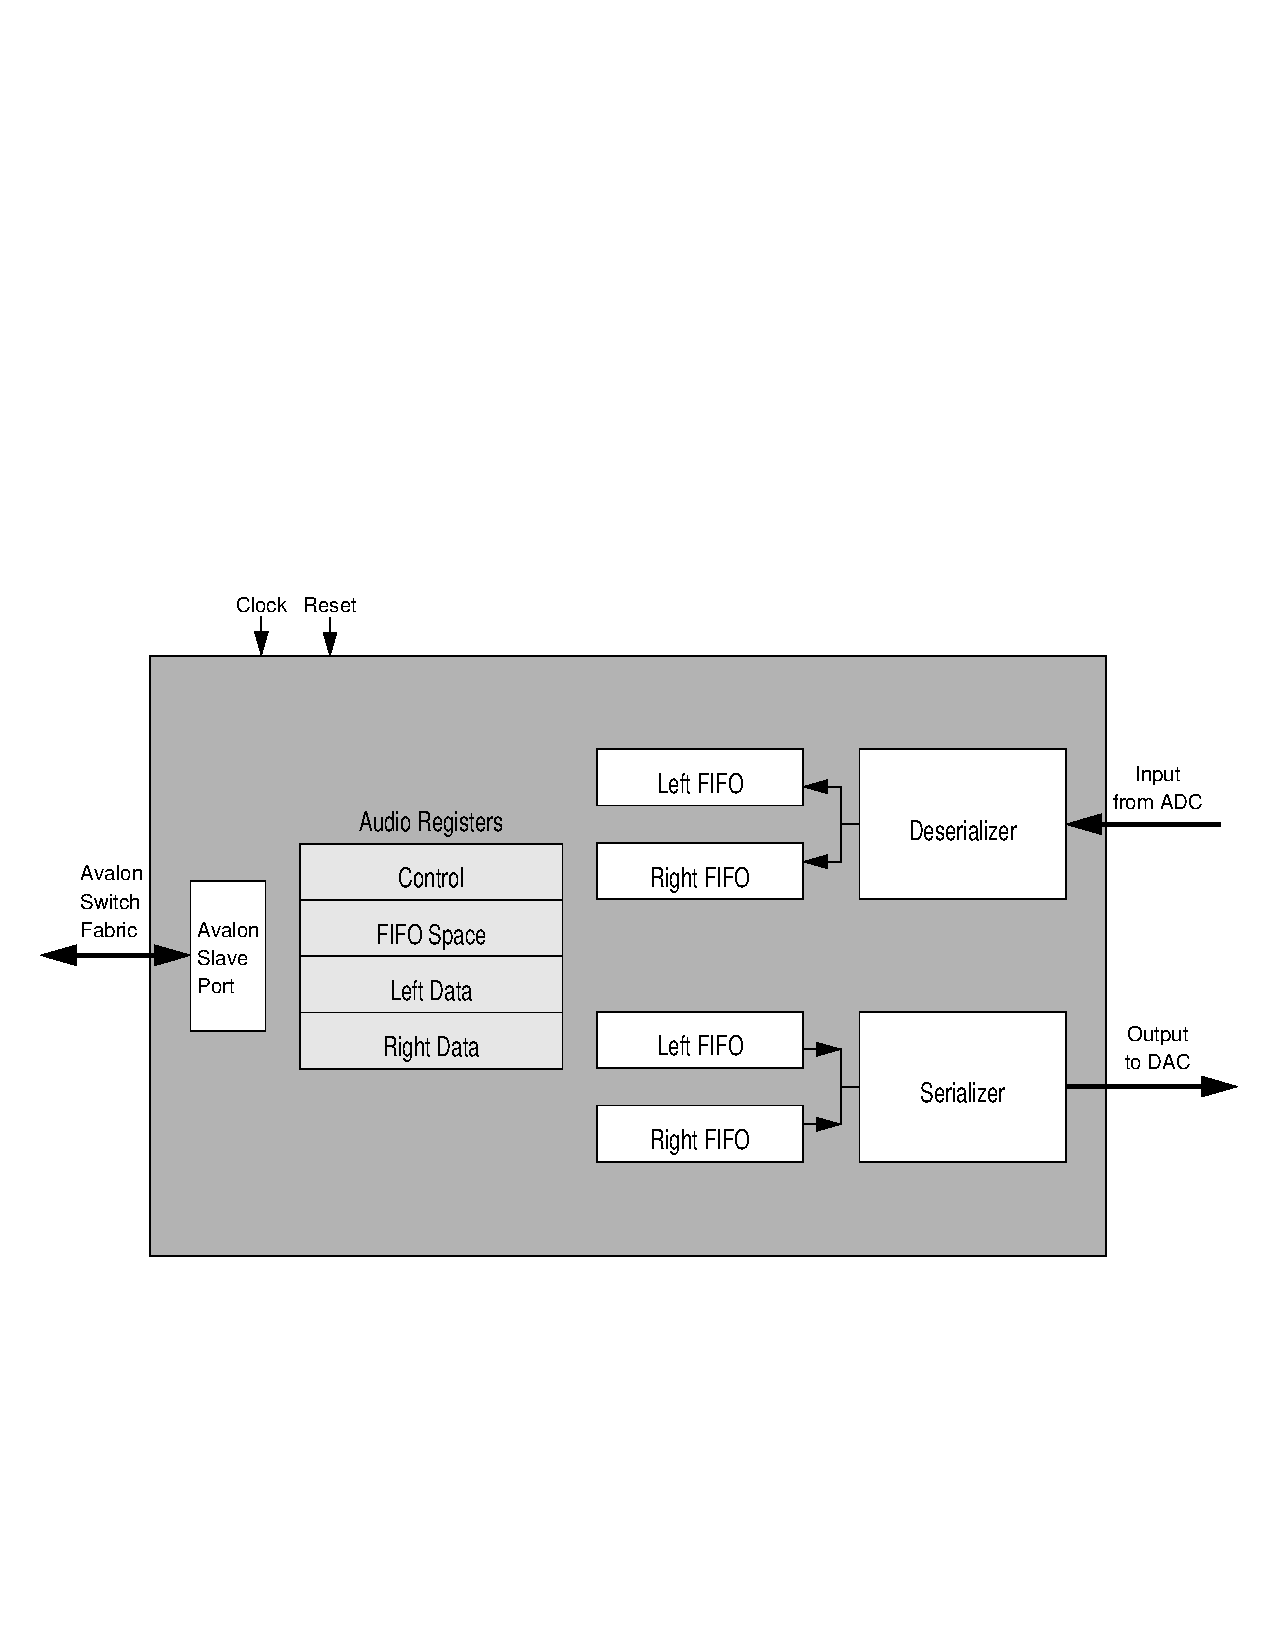
\includegraphics[width=0.9\textwidth]{fig/blockdiagram_mm.pdf}
    \end{center}
    \caption{Block diagram for Audio core with Memory-Mapped Interface}
    \label{fig:blockdiagrammm}
\end{figure}

\begin{figure}[h]
    \begin{center}
        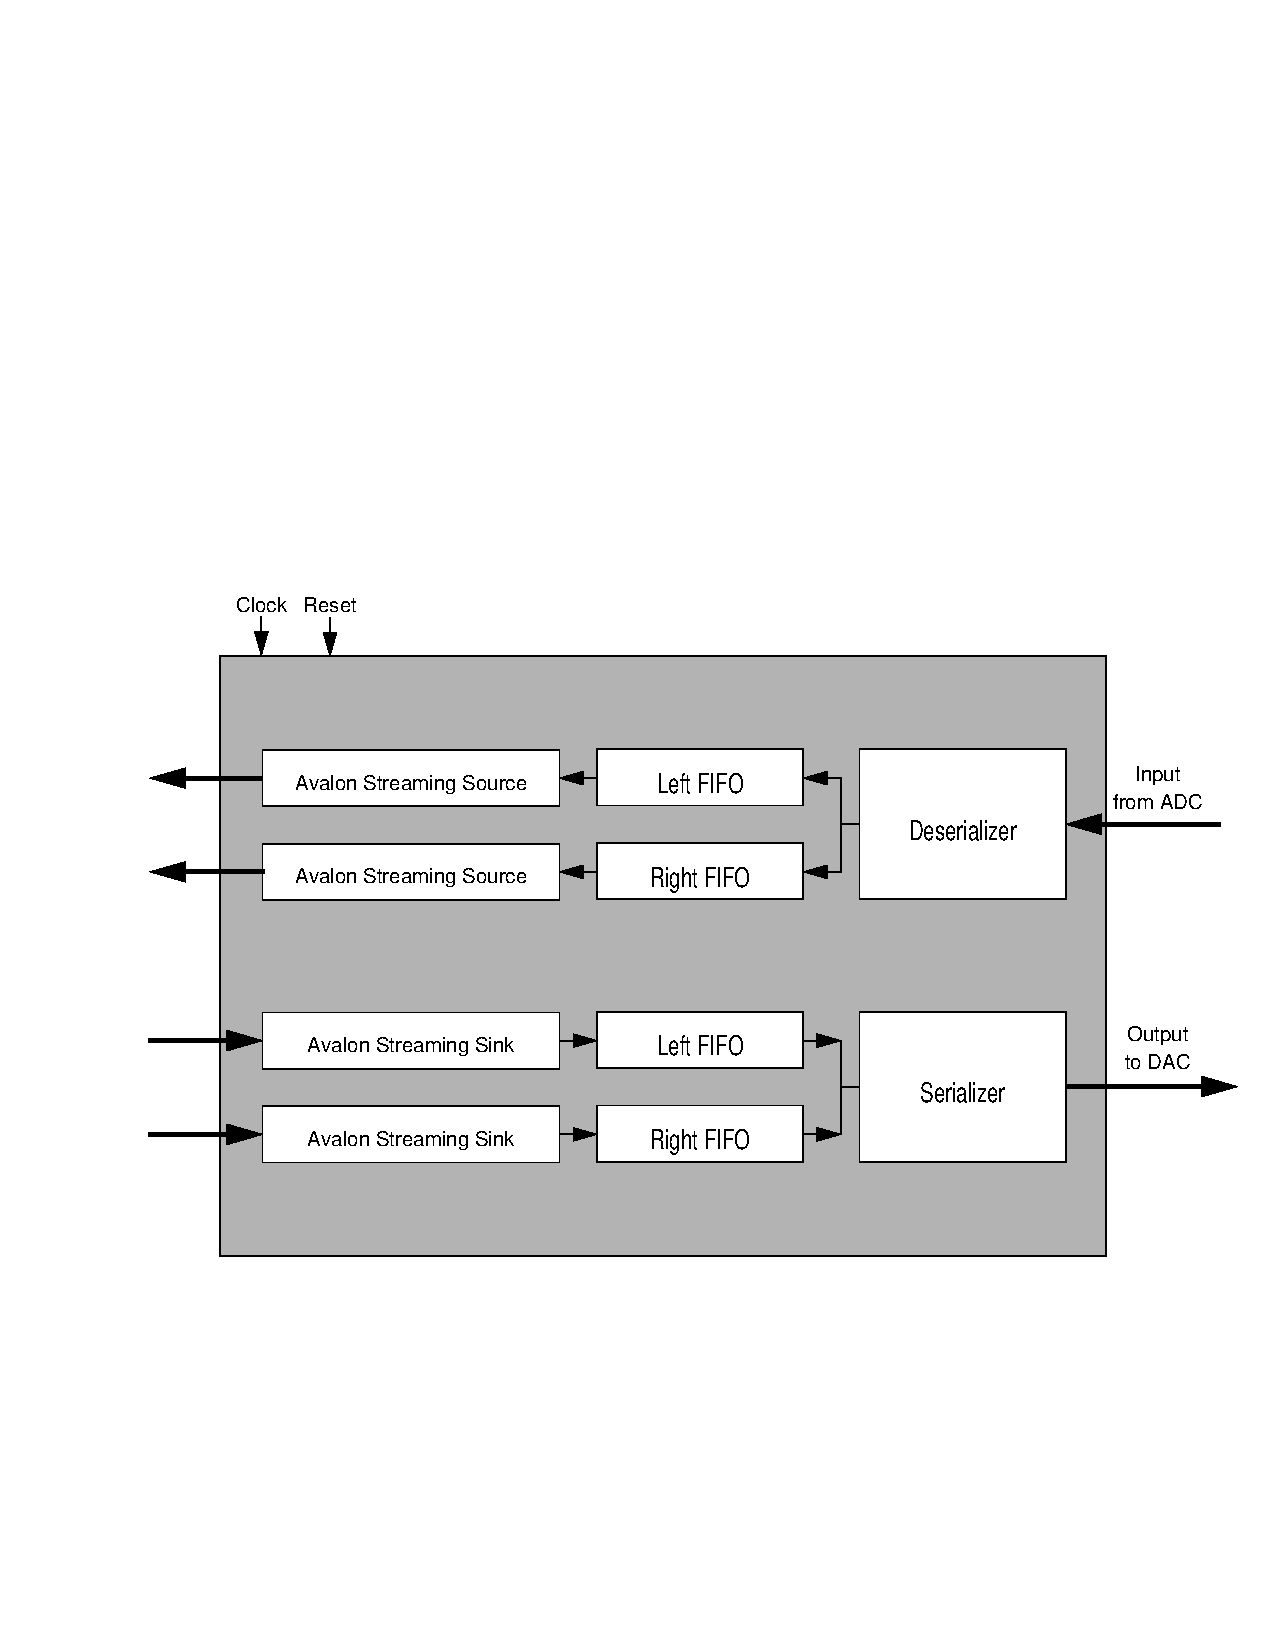
\includegraphics[width=0.9\textwidth]{fig/blockdiagram_st.pdf}
    \end{center}
    \caption{Block diagram for Audio core with Streaming Interface}
    \label{fig:blockdiagramst}
\end{figure}

The Audio core requires certain clock frequencies based on the sample rate of
the audio. The University Program's IP core, {\it Audio Clock for DE-series Boards},
can be use to provide those required clock frequencies. The Audio core also 
requires that the audio chip be initialized with some default values. The 
University Program's IO core, {\it Audio and Video Config}, provides the functionality
required to initialize the audio chip. Refer to the specific documentation for 
those cores for more information.

%\section{Device Support \& Tools}
%%    *  List the device families that the component supports. If all, say all.
%%    * If the core provides software for the Nios II processor, say so.
%%    * If there are any tools limitations, list them.
%The Audio core supports Altera's DE2/DE1 Development and Education Boards.

\newpage
\section{Instantiating the Core}
\label{sec:instantiation}
%This section is a flow-based description of how to create an instantiation of
%the core in SOPC Builder. The information to include in this section is
%dictated by the component configuration wizard. The following bullets are not
%an ordered outline of required information; they describe the type of
%information for this section.

%    * Describe what each GUI setting does. For each setting, use the exact
%    text/name as it appears in the GUI. The effects & properties of each
%    setting should be described here.
%    * If the option has a significant impact on LE or RAM usage, you can
%    include the comment, "This feature has a large impact on [ LE | RAM]
%    resource utilization." Avoid giving exact utilization numbers, because
%    they will inevitably change. It might be appropriate to give a range.
%    * For each GUI tab, include a section heading.
%    * For each group of settings on a tab, include a sub-heading.
%    * Do not include PTF descriptions, nor describe behavior in terms of PTF
%    variables. If the behavior of a feature depends on its PTF variable
%    setting, use the name of the setting as listed in the GUI.
%    * When writing the description for features, use the exact text as it appears in the GUI.
%          o If the text in the GUI is inappropriate, file an SPR to change it.
%    * Do not include a screenshot unless absolutely necessary.
%          o The appearance of GUIs change rapidly, which is problematic for
%          documentation. Refer to the exact text in the GUI, but do not
%          capture the exact pixels.
The Audio core can be instantiated in a system using Platform Designer or as a standalone 
component from the IP Catalog within the Quartus\textsuperscript{\textregistered} Prime software. 
Designers use the Audio core's \textbf{Configuration wizard} to specify the 
desired features. In the configuration wizard, the 
user can choose the interface type, whether it be memory-mapped or streaming. 
Also, the user can select whether to included only one or both of the audio in 
and/or audio out channels.
In addition, the \textsf{Data Width per Channel} 
can be specified. Data widths of 16, 20, 24, and 32 bits are supported. 
Remember to export the external\_interface connection to connect the core 
with the audio CODEC chip. It is recommended to set the \textsf{Avalon Type} to 
Memory-Mapped when connecting to a processor, otherwise set it to Streaming. 

{\leftpointright}
Altera recommends also instantiating the \textbf{\emph{Audio and Video Config}} 
core. This core automatically configures some required settings of the audio CODEC 
chip on the DE2/DE1 boards.
Refer to the \textbf{\emph{Audio and Video Config}} documentation for more 
information on properly intializing the audio codec.

{\leftpointright}
The user \textbf{\emph{must}} also instantiate the \textbf{{\em Audio Clock 
for DE-series Boards}} core and choose the proper audio clock 
setting for the Audio core. See \href{WM8731_WM8731L.pdf}{Wolfson* WM8731 audio 
CODEC Datasheet} in the "Audio Data Sampling Rates" section on page 37 for 
details on the relationship between sampling rate and clock frequency.
Note that the Audio and Video Config core provides settings for these values.

{\leftpointright}
When using the Memory-Mapped \textsf{Avalon Type} in Platform Designer, Altera recommends that the 
Audio core be used with the standard or fast 
versions of the Altera Nios II processor, so that a program 
running on the processor can keep up with the generation of audio data. If the 
economic version of the processor is used, then the 
program may run too slowly, and the audio may not be clear. In such, cases,
it may be possible to improve the audio clarity by selecting a 
lower sampling rate in the audio chip.

% NOTE: enable this section if applicable
%\section{Simulation Considerations}

\section{Software Programming Model}
% This section describes how the core appears from a software perspective.
% Memory components typically do not have a programming model, which is OK;
% just state that the component doesn't provide any software.

%\subsection{Nios II HAL Support}
%If the core supports the Nios II HAL, describe its functionality.
%    * Driver options (if applicable)
%    * ioctl() operations (if applicable) - List all available ioclt() options, and how they affect the behavior of the component.

%\subsection{Software Files}
%    *  List the .c & .h files provided by the component.
%    * For each file, give a short (one sentence) description of what it contains.

%\subsection{Programming with the Core}
%    *  If the core provides API functions, list them in a table with a short
%    description of each. (Complete descriptions of the functions are provided
%    in the API section.)
%    * If appropriate, provide examples of using the API functions to perform useful tasks.

\subsection{Register Map}
%    *  List the complete register map.
%    * Include a subsection for each register, which details the bits of the register.
%    * The register operations of some components are proprietary. In this
%    case, just say so and say that you're not going to say any more about the
%    register operations.

Software can control and communicate with the Audio core through four 32-bit
registers when using the Memory-Mapped \textsf{Avalon Type}. By writing or reading 
these registers, data can be fetched from the
CODEC's Analog-Digital Converter (ADC) or sent to the Digital-Analog Converter 
(DAC). Table~\hyperref[tab:regfiles]{1} shows the format of the registers.

\begin{table}[h]
    \centering
    \begin{tabular}{|c|l|c|c|c|c|c|c|c|c|c|c|c|}
        \hline
        \multicolumn{13}{|l|}{\it \textbf{{Table 1. Audio core register map}}}
        \\\hline
            \textbf{Offset}
            & \multicolumn{1}{c|}{\textbf{Register}}
            & \multirow{2}{*}{\textbf{R/W}}
            & \multicolumn{10}{c|}{\textbf{Bit Description}}
        \\\cline{4-13}
            \textbf{in bytes}
            & \multicolumn{1}{c|}{\textbf{Name}}
            &
            & \textbf{31\ldots24}
            & \textbf{23\ldots16}
            & \textbf{15\ldots10}
            & \textbf{9}
            & \textbf{8}
            & \textbf{7\ldots4}
            & \textbf{3}
            & \textbf{2}
            & \textbf{1}
            & \textbf{0}
        \\\hline
            0
            & \texttt{control}
            & RW
            & \multicolumn{3}{c|}{\footnotesize \it (1)}
            & WI
            & RI
            & {\footnotesize \it (1)}
            & CW
            & CR
            & WE
            & RE
        \\\hline
            4
            & \texttt{fifospace}
            & R
            & WS LC
            & WS RC
            & \multicolumn{3}{c|}{RA LC}
            & \multicolumn{5}{c|}{RA RC}
        \\\hline
            8
            & \texttt{leftdata}
            & RW {\footnotesize \it (2)}
            & \multicolumn{10}{c|}{Left Data}
        \\\hline
            12
            & \texttt{rightdata}
            & RW {\footnotesize \it (2)}
            & \multicolumn{10}{c|}{Right Data}
        \\\hline
                \multicolumn{13}{l}{}
        \\
                \multicolumn{13}{l}{\footnotesize \it{Notes on Table 1: }}
        \\
                \multicolumn{13}{l}{\footnotesize{(1) Reserved. Read values are undefined. Write zero.}}
        \\
                \multicolumn{13}{l}{\footnotesize{(2) Only reads incoming audio data and writes outgoing audio data.}}
    \end{tabular}
    \label{tab:regfiles}
\end{table}

\newpage
%The following sections introduces each register in details.
\subsubsection{\textit{Control} Register}
\begin{table}[h]
    \centering
    \begin{tabular}{|c|c|c|p{8.0cm}|}
        \hline
        \multicolumn{4}{|l|}{\it \textbf{Table 2. Control register bits}}
        \\\hline
            \textbf{Bit number}
            & \textbf{Bit name}
            & \textbf{Read/Write}
            & \textbf{Description}
        \\\hline
            0
            & RE
            & R/W
			& Interrupt-enable bit for read interrupts. If the RE bit is set to
			1 and both the left and right channel read FIFOs contain data, the
			Audio core generates an interrupt request (IRQ).
        \\\hline
            1
            & WE
            & R/W
			& Interrupt-enable bit for write interrupts. If the WE bit is set
			to 1 and both the left and right channel write FIFOs have space
			available for more data, the Audio core generates an interrupt 
			request (IRQ).
        \\\hline
            2
            & CR
            & R/W
            & Clears the Audio core's Input FIFOs, when the bit is 1. Clear 
			remains active until specifically set to zero.
        \\\hline
            3
            & CW
            & R/W
            & Clears the Audio core's Output FIFOs, when the bit is 1. Clear 
			remains active until specifically set to zero.
        \\\hline
            8
            & RI
            & R
            & Indicates that a read interrupt is pending.
        \\\hline
            9
            & WI
            & R
            & Indicates that a write interrupt is pending.
        \\\hline
    \end{tabular}
    \label{tab:control_reg}
\end{table}

\subsubsection{\textit{Fifospace} Register}
The \texttt{fifospace} register fields WSLC ($b_{31-24}$) and WSRC
($b_{23-16}$) indicate the number of words available (i.e., the amount of empty 
space) for outgoing data in the left and right channel FIFOs, respectively, 
while RALC ($b_{15-8}$) and RARC
($b_{7-0}$) indicate the number of words of incoming audio data in the left and
right channel FIFOs, respectively. When all of the outgoing and incoming FIFOs
are empty, the fifospace register will hold WSLC = WSRC = 128, and RALC = RARC = 0.

\subsubsection{\textit{Leftdata} Register}
The \texttt{leftdata} register is readable only for Audio In and writable only
for Audio Out.  It stores the data coming from or going to the left channel.
The data is always flush right, i.e., the LSB is $b_0$ of the \texttt{leftdata}
register.

\subsubsection{\textit{Rightdata} Register}
The \texttt{rightdata} register is readable only for Audio In and writable only
for Audio Out. It stores the data coming from or going to the right channel.
The data is always flush right, i.e., the LSB is $b_0$ of the
\texttt{rightdata} register.

\subsection{Interrupt Behavior}
The Audio core produces a read interrupt when either of the read FIFOs are 
filled to 75\% or more. The interrupt is cleared when the FIFO becomes less than 
75\% full. Also, it produces a write interrupt when either of the write FIFOs 
have available space of 75\% or more. The interrupt is cleared when the FIFO 
becomes less than 75\% empty. The Audio core generates an interrupt when 
either of these individual interrupt conditions are pending and enabled.

% If the component has and IRQ output, describe any specific points about how the IRQ must be serviced.

%\subsection{Accessing the Registers}
%    *  List all the #defines that this component includes in the system.h file.
%    * Specifically, list all the defined IO macros for reading/writing the registers.

\subsection{Device Driver for the Nios\textsuperscript{\textregistered} II Processor}
For use with the Nios II processor, the Audio core is packaged with C-language 
functions accessible through the
\href{http://www.altera.com/literature/hb/nios2/n2sw_nii5v2_02.pdf}{hardware
abstraction layer (HAL)}. These functions implement basic operations
for the Audio core. 

To use the functions, the C code must include the statement:

\qquad\texttt{\#include "altera\_up\_avalon\_audio.h"}

An example of C code that uses the Audio core is given at the end of this section.

%\subsection{Audio core Functions}
%\input{alt__up__audio_8h}
\subsubsection{alt\_up\_audio\_open\_dev}
\begin{tabular}[ht]{lp{11cm}}
	\textbf{Prototype:}
	&
	\texttt{alt\_up\_audio\_dev* alt\_up\_audio\_open\_dev(const char *name)} 
	\\
	\textbf{Include:}
	&
	{\tt <altera\_up\_avalon\_audio.h>}
	\\
	{\textbf{Parameters:}}
	&
	\texttt{{name}}
	 -- the audio component name in Platform Designer. 
	\\
	\textbf{Returns:}
	& The corresponding device structure, or NULL if the device is not found
	\\
	\textbf{Description:}
	& Opens the audio device specified by {\it name} (default "/dev/audio/").\\
\end{tabular}
\vfill

\subsubsection{alt\_up\_audio\_enable\_read\_interrupt}
\begin{tabular}[ht]{lp{11cm}}
	\textbf{Prototype:}
	&
	\texttt{void alt\_up\_audio\_enable\_read\_interrupt(alt\_up\_audio\_dev *audio)} 
	\\
	\textbf{Include:}
	&
	{\tt <altera\_up\_avalon\_audio.h>}
	\\
	{\textbf{Parameters:}}
	&
	\texttt{{audio}}
	 -- the audio device structure 
	\\
	\textbf{Returns:}
	& nothing
	\\
	\textbf{Description:}
	& Enable read interrupts for the Audio Core.\\
\end{tabular}
\vfill

\subsubsection{alt\_up\_audio\_disable\_read\_interrupt}
\begin{tabular}[ht]{lp{11cm}}
	\textbf{Prototype:}
	&
	\texttt{void alt\_up\_audio\_disable\_read\_interrupt(alt\_up\_audio\_dev *audio)} 
	\\
	\textbf{Include:}
	&
	{\tt <altera\_up\_avalon\_audio.h>}
	\\
	{\textbf{Parameters:}}
	&
	\texttt{{audio}}
	 -- the audio device structure 
	\\
	\textbf{Returns:}
	& nothing
	\\
	\textbf{Description:}
	& Disable read interrupts for the Audio Core.\\
\end{tabular}
\vfill

\subsubsection{alt\_up\_audio\_enable\_write\_interrupt}
\begin{tabular}[ht]{lp{11cm}}
	\textbf{Prototype:}
	&
	\texttt{void alt\_up\_audio\_enable\_write\_interrupt(alt\_up\_audio\_dev *audio)} 
	\\
	\textbf{Include:}
	&
	{\tt <altera\_up\_avalon\_audio.h>}
	\\
	{\textbf{Parameters:}}
	&
	\texttt{{audio}}
	 -- the audio device structure 
	\\
	\textbf{Returns:}
	& nothing
	\\
	\textbf{Description:}
	& Enable write interrupts for the Audio Core.\\
\end{tabular}
\vfill

\subsubsection{alt\_up\_audio\_disable\_write\_interrupt}
\begin{tabular}[ht]{lp{11cm}}
	\textbf{Prototype:}
	&
	\texttt{void alt\_up\_audio\_disable\_write\_interrupt(alt\_up\_audio\_dev *audio)} 
	\\
	\textbf{Include:}
	&
	{\tt <altera\_up\_avalon\_audio.h>}
	\\
	{\textbf{Parameters:}}
	&
	\texttt{{audio}}
	 -- the audio device structure 
	\\
	\textbf{Returns:}
	& nothing
	\\
	\textbf{Description:}
	& Disable the read interrupts for the Audio Core.\\
\end{tabular}
\vfill

\subsubsection{alt\_up\_audio\_read\_interrupt\_pending}
\begin{tabular}[ht]{lp{11cm}}
	\textbf{Prototype:}
	&
	\texttt{int alt\_up\_audio\_read\_interrupt\_pending(alt\_up\_audio\_dev *audio)} 
	\\
	\textbf{Include:}
	&
	{\tt <altera\_up\_avalon\_audio.h>}
	\\
	{\textbf{Parameters:}}
	&
	\texttt{{audio}}
	 -- the audio device structure 
	\\
	\textbf{Returns:}
	& 1 if read interrupt is pending, else 0
	\\
	\textbf{Description:}
	& Check if read interrupt pending for the Audio Core.\\
\end{tabular}
\vfill

\subsubsection{alt\_up\_audio\_write\_interrupt\_pending}
\begin{tabular}[ht]{lp{11cm}}
	\textbf{Prototype:}
	&
	\texttt{int alt\_up\_audio\_write\_interrupt\_pending(alt\_up\_audio\_dev *audio)} 
	\\
	\textbf{Include:}
	&
	{\tt <altera\_up\_avalon\_audio.h>}
	\\
	{\textbf{Parameters:}}
	&
	\texttt{{audio}}
	 -- the audio device structure 
	\\
	\textbf{Returns:}
	& 1 if write interrupt is pending, else 0
	\\
	\textbf{Description:}
	& Check if write interrupt pending for the Audio Core.\\
\end{tabular}
\vfill

\subsubsection{alt\_up\_audio\_reset\_audio\_core}
\begin{tabular}[ht]{lp{11cm}}
	\textbf{Prototype:}
	&
	\texttt{void alt\_up\_audio\_reset\_audio\_core(alt\_up\_audio\_dev *audio)} 
	\\
	\textbf{Include:}
	&
	{\tt <altera\_up\_avalon\_audio.h>}
	\\
	{\textbf{Parameters:}}
	&
	\texttt{{audio}}
	 -- the audio device structure 
	\\
	\textbf{Returns:}
	& nothing
	\\
	\textbf{Description:}
	& Reset the Audio Core by clearing read and write FIFOs for left and right channels.\\
\end{tabular}
\vfill

\subsubsection{alt\_up\_audio\_read\_fifo\_avail}
\begin{tabular}[ht]{lp{11cm}}
	\textbf{Prototype:}
	&
	\texttt{unsigned int alt\_up\_audio\_read\_fifo\_avail(alt\_up\_audio\_dev *audio, int channel)} 
	\\
	\textbf{Include:}
	&
	{\tt <altera\_up\_avalon\_audio.h>}
	\\
	{\textbf{Parameters:}}
	&
	\texttt{{audio}}
	 -- the audio device structure 
	\\
	&
	\texttt{{channel}}
	 -- left or right channel selection 
	\\
	\textbf{Returns:}
	& number of words available
	\\
	\textbf{Description:}
	& provides number of words of data available in the incoming FIFO for {\it channel} \\
\end{tabular}
\vfill

\subsubsection{alt\_up\_audio\_record\_r}
\begin{tabular}[ht]{lp{11cm}}
	\textbf{Prototype:}
	&
	\texttt{unsigned int alt\_up\_audio\_record\_r(alt\_up\_audio\_dev *audio, unsigned int *buf, int len)} 
	\\
	\textbf{Include:}
	&
	{\tt <altera\_up\_avalon\_audio.h>}
	\\
	{\textbf{Parameters:}}
	&
	\texttt{{audio}}
	 -- the audio device structure 
	\\
	&
	\texttt{{buf}}
	 -- the pointer to the allocated memory for storing audio data. Size of buf should be no smaller than len words. 
	\\
	&
	\texttt{{len}}
	 -- the number of data in words to read from the input FIFO 
	\\
	\textbf{Returns:}
	& The total number of words read.
	\\
	\textbf{Description:}
	& Read len words of data from right input FIFO, if the FIFO is above a threshold, and store data to where buf points.\\
\end{tabular}
\vfill

\subsubsection{alt\_up\_audio\_record\_l}
\begin{tabular}[ht]{lp{11cm}}
	\textbf{Prototype:}
	&
	\texttt{unsigned int alt\_up\_audio\_record\_l(alt\_up\_audio\_dev *audio, unsigned int *buf, int len)} 
	\\
	\textbf{Include:}
	&
	{\tt <altera\_up\_avalon\_audio.h>}
	\\
	{\textbf{Parameters:}}
	&
	\texttt{{audio}}
	 -- the audio device structure 
	\\
	&
	\texttt{{buf}}
	 -- the pointer to the allocated memory for storing audio data. Size of buf should be no smaller than len words. 
	\\
	&
	\texttt{{len}}
	 -- the number of data in words to read from the input FIFO 
	\\
	\textbf{Returns:}
	& The total number of words read.
	\\
	\textbf{Description:}
	& Read len words of data from left input FIFO, if the FIFO is above a threshold, and store data to where buf points.\\
\end{tabular}
\vfill
\subsubsection{alt\_up\_audio\_write\_fifo\_space}
\begin{tabular}[ht]{lp{11cm}}
	\textbf{Prototype:}
	&
	\texttt{unsigned int alt\_up\_audio\_write\_fifo\_space(alt\_up\_audio\_dev *audio, int channel)} 
	\\
	\textbf{Include:}
	&
	{\tt <altera\_up\_avalon\_audio.h>}
	\\
	{\textbf{Parameters:}}
	&
	\texttt{{audio}}
	 -- the audio device structure 
	\\
	&
	\texttt{{channel}}
	 -- left or right channel enum 
	\\
	\textbf{Returns:}
	& number of words available
	\\
	\textbf{Description:}
	& provides the amount of empty space in the outgoing FIFO for {\it channel} \\
\end{tabular}
\vfill

\subsubsection{alt\_up\_audio\_play\_r}
\begin{tabular}[ht]{lp{11cm}}
	\textbf{Prototype:}
	&
	\texttt{unsigned int alt\_up\_audio\_play\_r(alt\_up\_audio\_dev *audio, unsigned int *buf, int len)} 
	\\
	\textbf{Include:}
	&
	{\tt <altera\_up\_avalon\_audio.h>}
	\\
	{\textbf{Parameters:}}
	&
	\texttt{{audio}}
	 -- the audio device structure 
	\\
	&
	\texttt{{buf}}
	 -- the pointer to the data to be written. Size of buf should be no smaller than len words. 
	\\
	&
	\texttt{{len}}
	 -- the number of data in words to be written into the output FIFO 
	\\
	\textbf{Returns:}
	& The total number of data written.
	\\
	\textbf{Description:}
	& Write len words of data into right output FIFO, if space available in FIFO is above a threshold.\\
\end{tabular}
\vfill

\subsubsection{alt\_up\_audio\_play\_l}
\begin{tabular}[ht]{lp{11cm}}
	\textbf{Prototype:}
	&
	\texttt{unsigned int alt\_up\_audio\_play\_l(alt\_up\_audio\_dev *audio, unsigned int *buf, int len)} 
	\\
	\textbf{Include:}
	&
	{\tt <altera\_up\_avalon\_audio.h>}
	\\
	{\textbf{Parameters:}}
	&
	\texttt{{audio}}
	 -- the audio device structure 
	\\
	&
	\texttt{{buf}}
	 -- the pointer to the data to be written. Size of buf should be no smaller than len words. 
	\\
	&
	\texttt{{len}}
	 -- the number of data in words to be written into the output FIFO 
	\\
	\textbf{Returns:}
	& The total number of data written.
	\\
	\textbf{Description:}
	& Write len words of data into left output FIFO, if space available in FIFO is above a threshold.\\
\end{tabular}
\vfill

\subsubsection{alt\_up\_audio\_read\_fifo}
\begin{tabular}[ht]{lp{11cm}}
	\textbf{Prototype:}
	&
	\texttt{int alt\_up\_audio\_read\_fifo(alt\_up\_audio\_dev *audio, unsigned int *buf, int len, int channel)} 
	\\
	\textbf{Include:}
	&
	{\tt <altera\_up\_avalon\_audio.h>}
	\\
	{\textbf{Parameters:}}
	&
	\texttt{{audio}}
	 -- the audio device structure 
	\\
	&
	\texttt{{buf}}
	 -- the pointer to the allocated memory for storing audio data. Size of {\it buf} should be no smaller than {\it len} words. 
	\\
	&
	\texttt{{len}}
	 -- the number of data in words to read from each input FIFO 
	\\
	&
	\texttt{{channel}}
	 -- left or right channel selection 
	\\
	\textbf{Returns:}
	& The total number of words read.
	\\
	\textbf{Description:}
	& Read {\it len} words of data from left input FIFO or right input FIFO, and store data to where {\it buf} points.\\
\end{tabular}
\vfill

\subsubsection{alt\_up\_audio\_write\_fifo}
\begin{tabular}[ht]{lp{11cm}}
	\textbf{Prototype:}
	&
	\texttt{int alt\_up\_audio\_write\_fifo(alt\_up\_audio\_dev *audio, unsigned int *buf, int len, int channel)} 
	\\
	\textbf{Include:}
	&
	{\tt <altera\_up\_avalon\_audio.h>}
	\\
	{\textbf{Parameters:}}
	&
	\texttt{{audio}}
	 -- the audio device structure 
	\\
	&
	\texttt{{buf}}
	 -- the pointer to the data to be written. Size of {\it buf} should be no smaller than {\it len} words. 
	\\
	&
	\texttt{{len}}
	 -- the number of data in words to be written into each output FIFO 
	\\
	&
	\texttt{{channel}}
	 -- left or right channel selector 
	\\
	\textbf{Returns:}
	& The total number of data written.
	\\
	\textbf{Description:}
	& Write {\it len} words of data from {\it buf} to the left or right output FIFOs.\\
\end{tabular}
\vfill

\subsubsection{alt\_up\_audio\_read\_fifo\_head}
\begin{tabular}[ht]{lp{11cm}}
	\textbf{Prototype:}
	&
	\texttt{unsigned int alt\_up\_audio\_read\_fifo\_head(alt\_up\_audio\_dev *audio, int channel)} 
	\\
	\textbf{Include:}
	&
	{\tt <altera\_up\_avalon\_audio.h>}
	\\
	{\textbf{Parameters:}}
	&
	\texttt{{audio}}
	 -- the audio device structure 
	\\
	&
	\texttt{{channel}}
	 -- left or right channel selection 
	\\
	\textbf{Returns:}
	& the word read
	\\
	\textbf{Description:}
	& Read one data word from left input FIFO or right input FIFO.\\
\end{tabular}
\vfill

\subsubsection{alt\_up\_audio\_write\_fifo\_head}
\begin{tabular}[ht]{lp{11cm}}
	\textbf{Prototype:}
	&
	\texttt{void alt\_up\_audio\_write\_fifo\_head(alt\_up\_audio\_dev *audio, unsigned int data, int channel)} 
	\\
	\textbf{Include:}
	&
	{\tt <altera\_up\_avalon\_audio.h>}
	\\
	{\textbf{Parameters:}}
	&
	\texttt{{audio}}
	 -- the audio device structure 
	\\
	&
	\texttt{{data}}
	 -- the data word to be written 
	\\
	&
	\texttt{{channel}}
	 -- left or right channel selector 
	\\
	\textbf{Returns:}
	& nothing
	\\
	\textbf{Description:}
	& Write one data word to the left or right output FIFOs.\\
\end{tabular}
\vfill



\newpage
\subsubsection{Audio core C Example using Device Drivers }

\begin{figure}[h!]
\begin{center}
\begin{minipage}[t]{12.5 cm}
\begin{tabbing}
/\=*****\=*****\=*****\=*****\=*****\=*****\=*****\=*****\=*****\=*********************************\=\kill
\>\#include "altera\_up\_avalon\_audio.h"\\
\>\\
\>{\bf int} main({\bf void})\\
\>\{\\
\>\>alt\_up\_audio\_dev * audio\_dev;\\
\>\\
\>\>/* used for audio record/playback */\\
\>\>{\bf unsigned int} l\_buf;\\
\>\>{\bf unsigned int} r\_buf;\\
\>\\
\>\>// open the Audio port\\
\>\>audio\_dev = alt\_up\_audio\_open\_dev ("/dev/Audio");\\
\>\>{\bf if} ( audio\_dev == NULL)\\
\>\>\>alt\_printf ("Error: could not open audio device \textbackslash n");\\
\>\>{\bf else}\\
\>\>\>alt\_printf ("Opened audio device \textbackslash n");\\
\>\\
\>\>/* read and echo audio data */\\
\>\>{\bf while}(1)\\
\>\>\{\\
\>\>\>{\bf int} fifospace = alt\_up\_audio\_read\_fifo\_avail (audio\_dev, ALT\_UP\_AUDIO\_RIGHT);\\
\>\>\>{\bf if} ( fifospace > 0 ) 	// check if data is available \\
\>\>\>\{\\
\>\>\>\>// read audio buffer\\
\>\>\>\>alt\_up\_audio\_read\_fifo (audio\_dev, \&(r\_buf), 1, ALT\_UP\_AUDIO\_RIGHT);\\
\>\>\>\>alt\_up\_audio\_read\_fifo (audio\_dev, \&(l\_buf), 1, ALT\_UP\_AUDIO\_LEFT);\\
\>\\
\>\>\>\>// write audio buffer\\
\>\>\>\>alt\_up\_audio\_write\_fifo (audio\_dev, \&(r\_buf), 1, ALT\_UP\_AUDIO\_RIGHT);\\
\>\>\>\>alt\_up\_audio\_write\_fifo (audio\_dev, \&(l\_buf), 1, ALT\_UP\_AUDIO\_LEFT);\\
\>\>\>\}\\
\>\>\}\\
\>\}\\
\end{tabbing}
\end{minipage}
\end{center}
	\vspace{-0.33in}\caption{An example of C with Device Driver Support code that uses Audio Core.}
   \label{fig:HAL_Audio_Example}
\end{figure}
\pagebreak
\clearpage
\newpage



%\section{Hardware Revision History}
%\section{Software Revision History}
%\section{Document Revision History}
\input{\commonPath/Docs/copyright.tex}
\end{document}
